\chapter{Parallel computing architectures}\label{chap:parallelArchitectures}
                                                                                                                                                                                                                                                                                                                                                                                                                                                                                                                                                                                                                                                                                                                                                                                                                                                                                                                                                                                                                                                                                                                                                                                                                                                                                                                                                                                                                                                                                                                                                                                                                                                                                                                                                                                                                                                                                                                                                                                                                                                                                                                                                                                                                                                                                                                                                                                                                                                                                                                                                                                                                                                                                                                                                                                                                                                                                                                                                              
\section{Introduction}
Parallel computing has a tremendous impact on  various areas, raging from
scientific computation or simulation, commercial and industrial application and
data mining. Lot of effort has put during these years in order to try to
mitigate and overcome the limits regarding the sequential computer architecture.
In particular sequential architecture consist of three main components:
\begin{enumerate}
  \item Processor
  \item Memory
  \item Communication system (datapaths, usually buses)
\end{enumerate}
All three components present bottlenecks that limit the overall computing rate
of a system. Caches, low-latency high bandwidth and small capacity storage, for
example can hide latency of DRAM chips storing the fetched data and serving
subsequent requests of the same memory location\footnote{The fraction of the
data satisfied by the cache is called \textit{\textbf{hit rate}}.}. But one of
the most important innovation that addresses these bottlenecks is multiplicity
(in processor, memories and  dataphats) that allows to extend the class of
tractable problems with larger instances and more cases that can be handled. It
is so popular that even smartphones are multicore; Iphone 4S is 2-core, and nexus 4 is 4-core.
This multiplicity has been organized in several manners during
the years giving birth to a variety of architectures. Here a brief classification of the
most important ones.

\section{Architectures}
Classifying a parallel system is not a trivial task. Lots of definitions and
classifications have been proposed in years, mostly based on their hardware
configuration or logical approach in handling and implementing the parallelism.
\subsection{Classical classification - Flynn's taxonomy}
The classification is based on the notion of  \textit{stream of information}.
Two types of information flow into the processor: instructions and data.
Conceptually they can be separated into two independent streams. A coarse
classification can be made taking in account only the number of instructions and
 data streams that a parallel machine can manage (see figure \ref{fig:parallelClassification1}).
That's how Flynn's taxonomy\cite{Flynn1972} classifies machines: according to
whether they have one or more streams of each type.

\begin{figure}
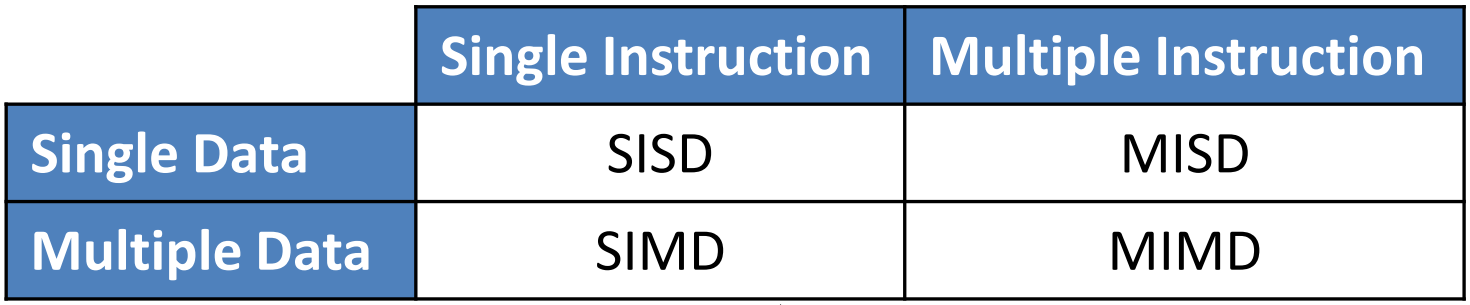
\includegraphics[scale=0.28]{./images/parallelClassification}
\caption[Parallel architecture classification]{Parallel architecture
classification.}
\label{fig:parallelClassification1}
\end{figure}


\begin{description}
\item[SISD:] \textit{\textbf{Single}} instruction \textit{\textbf{Single}}
data.\hfill\\
No parallelism in either instruction or data streams. Each arithmetic
instruction initiates an operation on a data item taken from a single stream of data elements (e.g. mainframes)
\item[SIMD:] \textit{\textbf{Single}} instruction
\textit{\textbf{Multiple}} data. \hfill \\ Data parallelism. The same
instruction is executed on a batch of different data. The control unit is
responsible for fetching and interpreting instructions. When it encounters an
arithmetic or other data processing instruction, it broadcasts the instruction
to all processing elements (PE), which then all perform the same operation. For
example, the instruction might be \textit{add R3,R0.}. Each PE would add the
contents of its own internal register R3 to its own R0. (e.g. stream
processors\footnote{Vector processing is performed on an SIMD machine by distributing
elements of vectors across all data memories.}.)
\item[MISD:] \textit{\textbf{Multiple}} instruction
\textit{\textbf{Single}} data. \hfill \\ Multiple instruction operating on the
same data stream. It is a class of system very unusual, mostly for fault-tolerance reasons.
\item[MIMD:] \textit{\textbf{Multiple}} instruction
\textit{\textbf{Multiple}} data. \hfill \\ Multiple instruction operating
independently on multiple data streams.
(e.g. most modern computers)
\end{description}



\subsection{Memory classification}
Architectures can be further organized by memory architecture and software
models. 
A first rough categorization can be obtained analyzing the memory layout:

\begin{figure}
\centering
\caption{Distributed memory architecture.}
\label{fig:distribuiteMemory}
\setlength{\fboxrule}{1pt}%
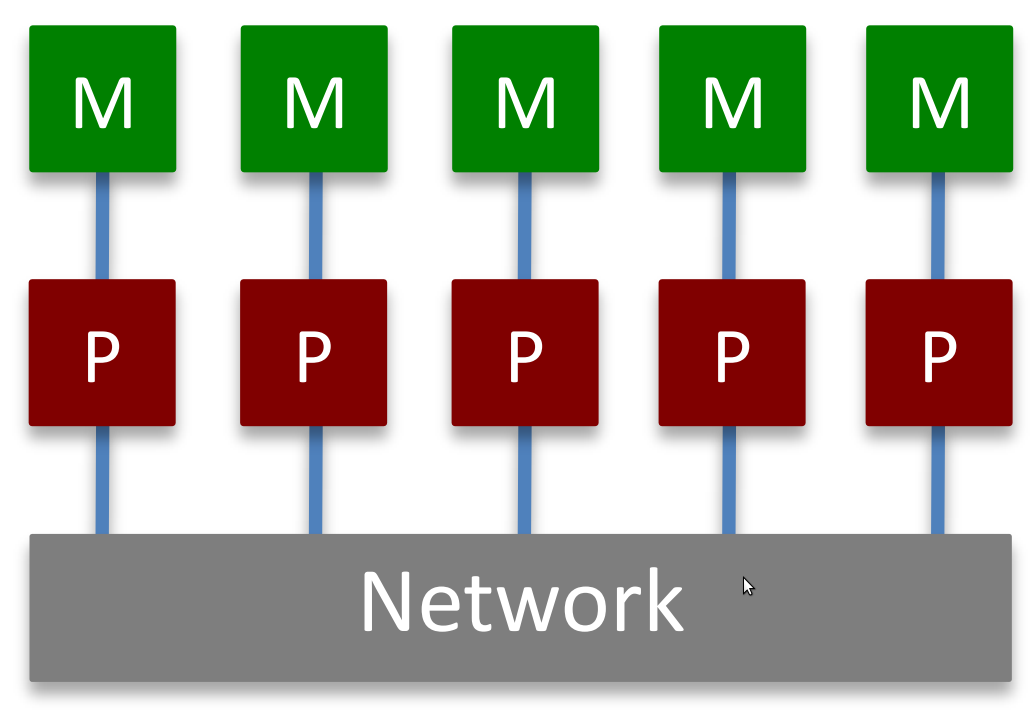
\includegraphics[scale=0.25]{./images/distribuitedMemory}
\end{figure}

\begin{description}
\item[Shared memory] \hfill \\ 
All the processors have in common the ability to access
all memory locations as global space, usually sharing them  via buses. Changes
in memory effected by one processor are visible to all the others. Historically
can be divided in :
		\begin{itemize}
  			\item UMA (Uniform Memory Access) : Identical processors with equal
  			access time to memory (see figure \ref{fig:UMA_NUMA}),
  			sometimes called CC-UMA acronym for Cache Coherent UMA, because the
  			hardware ensures that all the processor can see a memory modification
  			performed by one of them.
  			\item NUMA (Non Uniform Memory Access): Usually different groups
  			of processors (SMP, Symmetric multiprocessors\footnote{Group of processors
  			connected via buses. Usually they consist of not more than 32 processors.})
  			are connected, and processors belonging to different SMP can access memory
  			spaces of each others. As NUMA if is present a cache coherence mechanism
  			this architecture is called CC-NUMA.
  			
		\end{itemize}
		This memory architecture provides a user friendly perspective to memory and
		data sharing across processors, is fast due to the proximity of memory to
		CPUs, but it is not scalable because adding more CPUs can
		geometrically increase the traffic on the bus and for cache management. Is up
		to the programmer to ensure the correct accesses to global memory in order to
		avoid race-conditions.
		
		Coupled with this architecture many software solution can be used to program
		shared memory machines. The most used are:

\begin{itemize}
  \item Threads. Lightweight processes but with same PID (e.g. pthreads)
  \item A standard language with preprocessor directives to the compiler that is
  capable of converting the serial program in a parallel program without any (or
  very few) intervention by the programmer (e.g. OpenMP\footnote{Built on top
  of pthreads}, see example code \ref{code:OpenMPFOR} and
  \ref{code:OpenMPREDUCTION} at page \pageref{code:OpenMPFOR} for complete examples ).

\end{itemize}

\begin{figure}
\centering
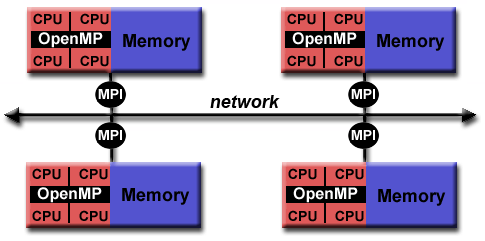
\includegraphics[scale=0.8]{./images/hybrid_model}
\caption{Hybrid memory architecture (Each processor is milti-core)}
\label{fig:hybridMemory}
\end{figure}

\item[Distributed Memory]
	Different systems, and hence, different processors connected via some
	kind of network (see figure \ref{fig:distribuiteMemory}) (usually high speed
	networks) and the memory space in one processor do not map to another processor. Each of them operate independently on its memory space,
	so changes are not reflected on memory spaces of the others. Explicit
	communication is required between processors and is like synchronization
	programmer's responsibility.
This architecture  is very scalable and there's not any overhead in maintaining
cache coherency but all the communication work rely on the programmer.

The most used paradigm for programming distributed memory machines is the
message passing\footnote{MPI is the \textit{de facto} industry standard for
message passing. Visit  \url{http://www.mpi-forum.org/}} for further
informations.

\item[Hybrid Systems] As the name suggest is a mix of the two architectures seen
before. Only a limited number of  processors, say N, have
access to a common pool of shared memory. These N processor are connected to the
others via network and each processor can consist of many cores.
A common example of a  programming model for hybrid system is the combination
of the message passing model (MPI) with the threads model (OpenMP) in which
\begin{inparaenum}[\itshape a\upshape)]
\item threads perform computationally intensive task, using local
\textbf{on-node} memory space and
\item communications between processes on different nodes occurs over network
using MPI (see figure\ref{fig:hybridMemory}).

\end{inparaenum} 
\end{description}


\begin{figure}
\centering
\setlength{\fboxrule}{0.5pt}%
\subfigure[UMA]{ \fbox{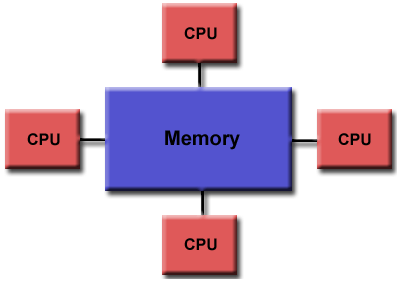
\includegraphics[scale=0.47]{./images/shared_mem}}}
\hfill
\subfigure[NUMA]{\fbox{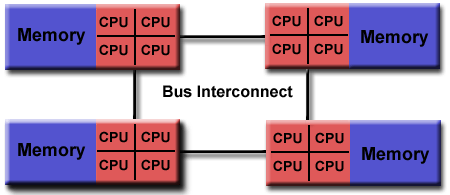
\includegraphics[scale=0.47]{./images/numa}}}
\hfill
\caption{Shared memory architectures.}
\label{fig:UMA_NUMA}
\end{figure}

\section{Network Topologies}
An important role is played, as seen before, by the interconnection network 
because provide mechanisms for data transfer between processing nodes.
Typically they consist of \textit{n} inputs and \textit{m} outputs and are built
in by switches and links (set of wires or fibers capable of carrying
information\footnote{Links may have different characteristics depending on
the material they are made of that can limit speed propagation of the signals
or the maximum length of the wire itself}).
\begin{figure}
\begin{center}
\caption{Start network topology}
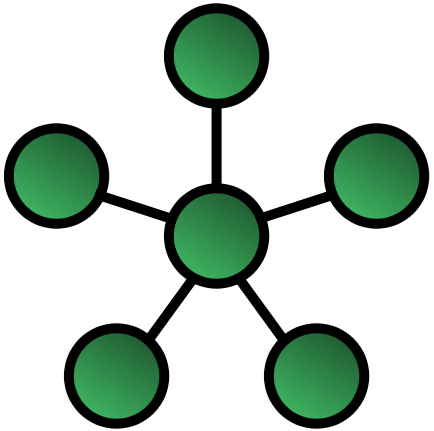
\includegraphics[scale=0.30]{./images/StartMesh}
\label{fig:starMesh}
\end{center}
\end{figure}
A first classification can be done considering only if the nodes are connected
directly to each others or not. In the first case the entire network consist of
point-to-point links and they are called \textbf{\textit{static}} or
\textbf{\textit{direct}} networks. On the other hand when the nodes are
connected to each others using switches we talk about \textbf{\textit{indirect}}
networks. Because communication is an important task in parallel computing,
the way the nodes are connected to each other is important and can influence
the overall performance of the system that is determined by the capabilities of
the network access devices, the level of control or fault tolerance desired, and
the cost associated with cabling or telecommunications circuits.
Networks topologies try to trade off cost and scalability with performance

\subsection{Bus-based networks}\label{bus-based}
The most simple family of topologies that give birth to the bus-based
networks. Each node is connected to a single shared medium that is common to all
the nodes. The most important advantage of bus is that the distance of two nodes is constant \textit{O}(1) and the cost scale linearly
as the number of nodes \textit{p}\footnote{The cost is usually associated with
the bus interface coupled with each node and is inexpensive to implement
compared to other topologies}.
A message from the source is broadcasted to all machines connected to the bus
and every machine ignore the message except for the intended address for the
message that accept the data. The low cost of implementing this topology if
tradeoff by the difficulties in managing it and plus, because of the bounded
bandwidth of buses, typical bus-based machine are limited to dozen of nodes.

\subsection{Completely connected networks}
In a completely-connected network, each node has a direct communication link to every other
node in the network. This kind of networks don't need any switching or
broadcasting mechanism because a node can send a message to another in a single
step, and interferences during the communication are completely prevented.
But completely connected network are not suitable for practical uses because of
the cost related to their implementation. The number of connection grows
quadratically \(O(p^2)\) with the number of the nodes (see figure
\ref{fig:completelyConnected}).
\[
c=\frac{n(n-1)}{2}
\]

\begin{figure}
\begin{center}
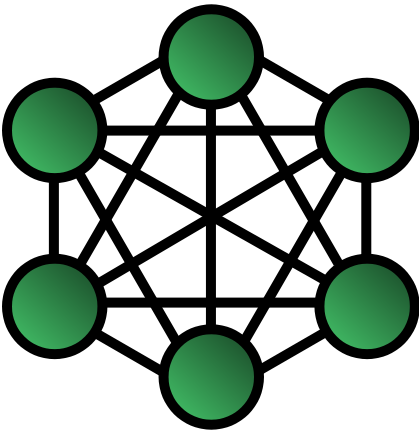
\includegraphics[scale=0.4]{./images/FullMesh}
\caption{Fully connected mesh network. 6 nodes and c=15 links}
\label{fig:completelyConnected}
\end{center}
\end{figure}



\subsection{Star-Connected Networks}

Star topology (see figure \ref{fig:starMesh}) every node is connected to
a central node that acts as the central processor (as server if we consider the
analogy with the LAN) . It is similar to the bus-based (see section \ref{bus-based}) network, because communication
between any pair of nodes is routed through the central processor (and the
latter is the shared medium the all the other nodes share) and because the
central processor is the bottleneck in this topology and also the single point
of failure (if this node goes down  the entire network stops to work).




\subsection{K-Meshes}


\begin{wrapfigure}{r}{0.4\textwidth}
\centering
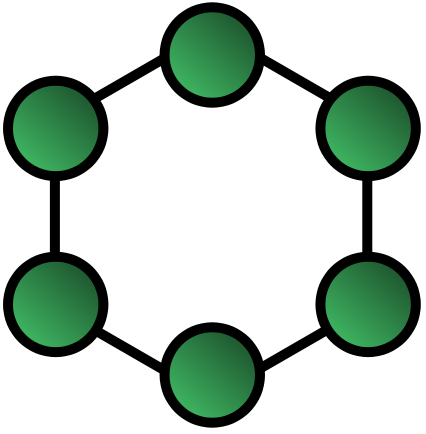
\includegraphics[scale=0.3]{./images/ring}
\caption{1-mesh ring topology}
\setlength{\fboxrule}{1pt}%
\label{fig:ring}
\end{wrapfigure}
Due to the large number of links in fully connected networks, sparser networks
are typically used to build parallel computers. A family of such networks spans the space of linear arrays and
hypercubes.
Linear array or ring are static network in which each node is connected with
other two (called neighbors, see figure \ref{fig:ring}).

The 2-D version of the ring topology is the 2-D torus (see figure
\ref{fig:torus}).
It consist of \(\sqrt{p}\) processor per each dimension, and each processor is connected to
four neighbors (ones whose indices differ in any dimension by one). 2-D or 3-D
meshes are very often used to build parallel machines because they are attractive from a
wiring standpoint (2-D mesh laid out in 2-D space) and because it naturally
maps a variety of computation ( matrices, 3-D weather modeling, structural
modeling, etc.). 



\begin{figure}
\caption{2D (a) and 3D (b) torus topologies.}
\label{fig:torus}
\centering
\setlength{\fboxrule}{0.5pt}%
\subfigure[2D]{ 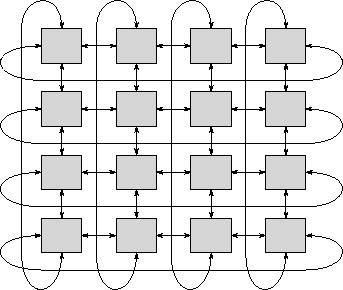
\includegraphics[scale=0.47]{./images/torus2D}}
\hfill
\subfigure[3D]{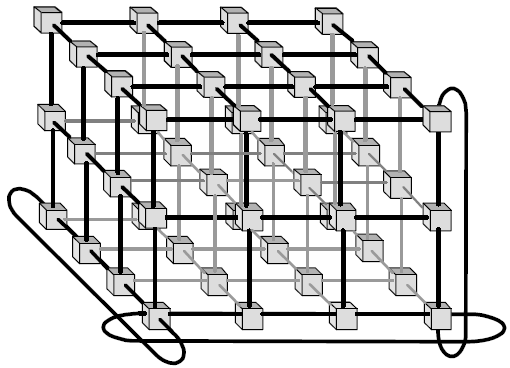
\includegraphics[scale=0.47]{./images/torus3D}}

\end{figure}

\subsection{Three based}
This type of network topology is based on a hierarchy of nodes. The highest
level of any tree network consists of a single node, the ``\textit{root}'' that
connects nodes (a fixed number referred to as the ``branching
factor''\footnote{If the branching factor is \(1\) the topology is called
linear.} of the tree) in the level below by point-to-point links. These lower
level nodes are also connected to nodes in the next level down. Tree networks
are not constrained to any number of levels, but as tree networks are a variant
of the bus network topology, they are prone to crippling network failures should
a connection in a higher level of nodes fail/suffer damage.
This topology exhibits good scalability and thanks to the different levels makes
fault identification and isolation easier but the maintenance may be an issue
when the network spans a great area.


